\documentclass[tikz]{standalone}

\usepackage{xcolor}
\usepackage{tikz}
\usepackage{pgfplots}
\usepackage{amsmath}



% \newcommand{\midlinewidth}{0.6pt}
\newcommand{\midlinewidth}{1.0pt}
\newcommand{\largelinewidth}{1.7pt}
\newcommand{\middist}{17pt}
\newcommand{\largedist}{40pt}
\newcommand{\smalldist}{17pt}

\definecolor{lacamdarklilac5} {RGB} {51, 10, 102}
\colorlet{lacamdarklilac4} {lacamdarklilac5!80!}
\colorlet{lacamdarklilac3} {lacamdarklilac5!60!}
\colorlet{lacamdarklilac2} {lacamdarklilac5!40!}
\colorlet{lacamdarklilac1} {lacamdarklilac5!20!}

\definecolor{lacamgold5} {RGB} {255, 87, 0}
\colorlet{lacamgold4} {lacamgold5!80!}
\colorlet{lacamgold3} {lacamgold5!60!}
\colorlet{lacamgold2} {lacamgold5!40!}
\colorlet{lacamgold1} {lacamgold5!20!}
\definecolor{gold1} {RGB} {255, 180, 0}
\definecolor{violet} {RGB} {119, 111, 178}
\definecolor{petroil2} {RGB} {36, 165, 175}
\definecolor{petroil4} {RGB} {30, 132, 149}
\definecolor{petroil6} {RGB} {23, 101, 115}
\definecolor{gold2} {RGB} {255, 130, 0}
\definecolor{gold4} {RGB} {250, 100, 0}
\definecolor{gold6} {RGB} {245, 90, 0}

\definecolor{lacamoil5}{rgb}{0.13, 0.67, 0.8}
\colorlet{lacamoil4} {lacamoil5!80!}
\colorlet{lacamoil3} {lacamoil5!60!}
\colorlet{lacamoil2} {lacamoil5!40!}
\colorlet{lacamoil1} {lacamoil5!20!}

\usepackage{tikz}
\usetikzlibrary{circuits.logic.US}
\usetikzlibrary{shapes.misc}
\usetikzlibrary{shapes.arrows}
\usetikzlibrary{arrows,shapes.geometric}
\usetikzlibrary{patterns,calc,backgrounds}
\usetikzlibrary{trees}

\tikzstyle{nnf}=[
  >=latex, thick, >=stealth, font=\small,auto,scale=0.9,every node/.style={scale=0.9}
]
\tikzstyle{nnfnode}=[
  line width=1.0pt, draw
]
\tikzstyle{nnfand}=[
  nnfnode, and gate, rotate=90
]
\tikzstyle{nnfor}=[
  nnfnode, or gate, rotate=90
]
\tikzstyle{nnf2or}=[
  nnfor, inputs=nn
]
\tikzstyle{nnf2and}=[
  nnfand, inputs=nn
]
\tikzstyle{nnf3or}=[
  nnfor, inputs=nnn, scale=0.75
]
\tikzstyle{nnf4and}=[
  nnfand, inputs=nnnn, scale=0.65
]
\tikzstyle{nnfedge}=[
    line width=0.9
]
\tikzstyle{nnfterm}=[
  draw,fill=gray!10,inner sep=2.5pt, font=\small
]
\definecolor{hotcolor}{rgb}{0.85,0.0,0.0}
\tikzstyle{hot}=[
  draw=hotcolor, line width=1.1pt
]
\tikzstyle{hotparam}=[
  text=hotcolor
]

\begin{document}
% \begin{figure*}[t!]
% \begin{subfigure}[t]{0.17\textwidth}
% \centering
% \scalebox{.9}{
% }
% \caption{A vtree}\label{fig: vtree}
% \end{subfigure}
% \begin{subfigure}[t]{0.37\textwidth}
% \centering
% \scalebox{0.67}{
    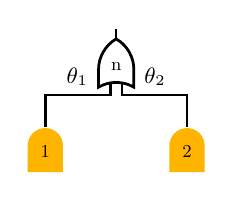
\begin{tikzpicture}[circuit logic US, nnf]

    \node (root) [nnf2or, scale=0.9] at ($(0.0, 0.0)$) {
    \rotatebox{-90}{n}
    }; 
    \node (and4) [nnf2and, scale=0.9,fill=gold1, draw=none] at ($(root) + (-1, -1.2)$) {
        \rotatebox{-90}{1}
    };
    \node (and5) [nnf2and, scale=0.9,fill=gold1, draw=none] at ($(root) + (1, -1.2)$) {
        \rotatebox{-90}{2}
    };
    
    \node (dummy) at ($(root) + (0.0, 0.4)$) {}; 
    \begin{scope}[on background layer]
        \draw [nnfedge] (and4.output) -- ++ (up: 0.45) -| (root.input 1)
                 node[pos=0.4,above left] {$\theta_1$};
        \draw [nnfedge] (and5.output) -- ++ (up: 0.45) -| (root.input 2)
                 node[pos=0.4,above right] {$\theta_2$};
        \draw [nnfedge] (root.output) -- (dummy);
    \end{scope}
    \end{tikzpicture}
% }
% \caption{A PSDD}\label{fig:PSDD}
% \end{subfigure}
% \begin{subfigure}[t]{0.45\textwidth}
% \centering
% \scalebox{.65}{
    % \begin{tikzpicture}[circuit logic US, nnf]

    % \node (root) [nnf2or, scale=0.9] at ($(0.0, 0.0)$) {
    %     \rotatebox{-90}{m}
    % }; 
    % \node (and4) [nnf2and, scale=0.9,fill=gold1, draw=none] at ($(root) + (-1, -1.2)$) {
    %     \rotatebox{-90}{3}
    % };
    % \node (and5) [nnf2and, scale=0.9,fill=gold1, draw=none] at ($(root) + (1, -1.2)$) {
    %     \rotatebox{-90}{4}
    % };
    
    % \node (dummy) at ($(root) + (0.0, 0.4)$) {}; 
    % \begin{scope}[on background layer]
    %     \draw [nnfedge] (and4.output) -- ++ (up: 0.45) -| (root.input 1)
    %              node[pos=0.4,above left] {$\phi_1$};
    %     \draw [nnfedge] (and5.output) -- ++ (up: 0.45) -| (root.input 2)
    %              node[pos=0.4,above right] {$\phi_2$};
    %     \draw [nnfedge] (root.output) -- (dummy);
    % \end{scope}
    % \end{tikzpicture}

\end{document}

%%% Local Variables:
%%% mode: latex
%%% TeX-master: t
%%% End:


%%% Local Variables:
%%% mode: latex
%%% TeX-master: t
%%% End:
